
%\documentclass[mathserif]{beamer}
\documentclass[handout]{beamer}
%\usetheme{Goettingen}
%\usetheme{Warsaw}
\usetheme{Singapore}



%\usetheme{Frankfurt}
%\usetheme{Copenhagen}
%\usetheme{Szeged}
%\usetheme{Montpellier}
%\usetheme{CambridgeUS}
%\usecolortheme{}
%\setbeamercovered{transparent}
\usepackage[english, activeacute]{babel}
\usepackage[utf8]{inputenc}
\usepackage{amsmath, amssymb}
\usepackage{dsfont}
\usepackage{graphics}
\usepackage{cases}
\usepackage{graphicx}
\usepackage{pgf}
\usepackage{epsfig}
\usepackage{amssymb}
\usepackage{multirow}	
\usepackage{amstext}
\usepackage[ruled,vlined,lined]{algorithm2e}
\usepackage{amsmath}
\usepackage{epic}
\usepackage{epsfig}
\usepackage{fontenc}
\usepackage{framed,color}
\usepackage{palatino, url, multicol}
%\algsetup{indent=2em}
\newcommand{\factorial}{\ensuremath{\mbox{\sc Factorial}}}
\newcommand{\BIGOP}[1]{\mathop{\mathchoice%
{\raise-0.22em\hbox{\huge $#1$}}%
{\raise-0.05em\hbox{\Large $#1$}}{\hbox{\large $#1$}}{#1}}}
\newcommand{\bigtimes}{\BIGOP{\times}}
\vspace{-0.5cm}
\title{Natural Language Processing \\ Vectors Space Model and Information Retrieval}
\vspace{-0.5cm}
\author[Felipe Bravo Márquez]{\footnotesize
%\author{\footnotesize  
 \textcolor[rgb]{0.00,0.00,1.00}{Felipe Bravo-Marquez}} 
  
 

\date{\today}

\begin{document}
\begin{frame}
\titlepage


\end{frame}

\begin{frame}\frametitle{Motivation}


  \begin{itemize}
   \item How does a search engine such as Duckduckgo or Google retrieve relevant documents from a given query?
   \item How can a company process the claims left by its users on its Web portals?
  \end{itemize}

These problems are studied in the following fields:

\begin{itemize}
 \item \emph{Information Retrieval}:  science of searching for information in  document collections.
 \item \emph{Text Mining}: automatic extraction of knowledge from text.
\end{itemize}

Both of them are closely related to NLP! (the borders between these fields are unclear).

\end{frame}

\begin{frame}\frametitle{Tokens and Types}
{\footnotesize
Tokenization: the task of splitting a sentence or document into pieces called \emph{tokens}. \\
Additional transformations can be employed such as the removal of special characters (e.g., punctuation), lowercasing, etc. ~\cite{manning2008}. 

\begin{block}{Example}
Input: I like human languages and programming languages.\\
Tokens: [I] [like] [human] [languages] [and] [programming] [languages]
\end{block}



\begin{block}{Types}
\begin{itemize}
 \item A \emph{type} is a class of \emph{token} containing a single sequence of characters.
\item They are obtained by identifying unique tokens within the document.
\end{itemize}

Types for the previous sentence: [I] [like] [human] [languages] [and] [programming]  \\
\center{The token \emph{languages} was repeated in the sentence.}
\end{block}



 }
\end{frame}

\begin{frame}\frametitle{Vocabulary Extraction }
\footnotesize{
\begin{itemize}
 \item A  \emph{term} is a normalized \emph{type}. 
 \item Normalization is the process of creating equivalence classes of different \emph{types}. This will become clear in the following slides.
 \item The vocabulary $V$, is the set of terms (normalized unique tokens) within a collection of documents or corpus $D$.
\end{itemize}
 
\begin{block}{Stopwords removal}
\begin{itemize}
 \item In order to reduce the size of the vocabulary and eliminate terms that do not provide much information, terms that occur with high frequency in the corpus are eliminated. 
 \item These terms are called \emph{stopwords} and include  articles, pronouns, prepositions and conjunctions. \\
Example: [a, an, and, any, has, do, don't, did, the, on].\footnote{Related concepts: function words, closed-class words.}
\end{itemize}

The removal of stopwords can be inconvenient in many NLP tasks!! 
\\ Example: I don't like pizza $=>$ pizza  ( ``I'', ``don't'', and ``like'' were removed)

\end{block}


}
 
\end{frame}


\begin{frame}\frametitle{Stemming}
\footnotesize{
A term normalization process in which terms are transformed to their root in order to reduce the size of the vocabulary. It is carried by applying word reduction rules. \\ Example: Porter's Algorithm.

\begin{figure}[h!]
	\centering
	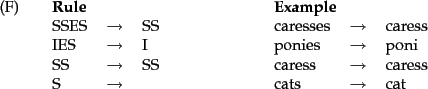
\includegraphics[scale=0.45]{pics/porter.png}
\end{figure}

 Example: $d$ = I like human languages and programming languages $=>$
I like human languag and program languag \footnote{\url{http://9ol.es/porter_js_demo.html}}

The vocabulary of document $d$ after removing stopwords and performing stemming:


\begin{table}
\centering
\begin{tabular}{c|c}
\hline
termId & value \\ 
\hline
t1 & human \\ 
t2 & languag \\ 
t3 & program\\ 
\hline
\end{tabular}
\end{table}

}
 
\end{frame}


\begin{frame}\frametitle{Lemmatization}
\footnotesize{

\begin{itemize}
\item Another term normalization strategy.
 \item It also transform words into their roots.
 \item It performs a morphological analysis using reference dictionaries (lookup tables) to create equivalence classes between \emph{types}.
\item For example, for the token \emph{studies}, a stemming rule would return the term \emph{studi}, while through lemmatization we would get the term \emph{study}\footnote{\url{https://blog.bitext.com/what-is-the-difference-between-stemming-and-lemmatization/}}. 

\end{itemize}





}
\end{frame}



\begin{frame}\frametitle{Zipf's law [1]}
\footnotesize{
\begin{itemize}
\item The Zipf's law, proposed by \emph{George Kingsley Zipf} in \cite{zipf1935}, is an empirical law about the frequency of terms within a collection of documents (\textbf{corpus}). 
\item It states that the frequency $f$ of a term in a corpus is inversely proportional to its $r$ ranking in a sorted frequency table:
\begin{equation}
	f = \frac{cf}{r^{\beta}}
\end{equation}
\item Where $cf$ is a constant dependent on the collection and $\beta > 0$ is a decay factor.
\item If $\beta = 1$, then $f$ follows exactly Zipf's law, otherwise it follows a Zipf-like distribution. 

\item The law relates to the principle of minimum effort. We often use a few words to write ideas.

\item The Zipf law is a type of power law distribution (long tail distributions)


\end{itemize}


}
 
\end{frame}


\begin{frame}\frametitle{Zipf's law [2]}
\footnotesize{

\begin{figure}[h!]
	\centering
	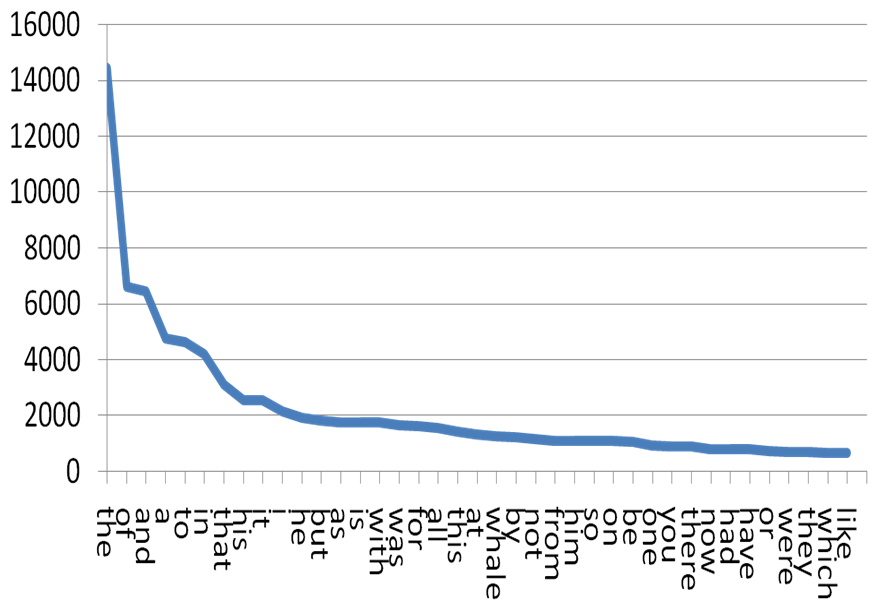
\includegraphics[scale=0.5]{pics/zipf1.png}
	\caption{Zipf's law}
\end{figure}
\begin{itemize}
 \item If we plot a $log-log$ graph, we obtain a straight line with slope  $-\beta^{-1}$.
 \item Listing the most frequent words of a corpus can be used to build a \emph{stopwords} list. 
\end{itemize}
}



 
\end{frame}

\begin{frame}\frametitle{Posting Lists and the Inverted Index}
{\footnotesize Let $D$ be a collection of documents  and $V$ the vocabulary of all terms extracted from the collection:

\begin{itemize}
 \item The posting list of a term is the list of all documents where the term appears at least once. Documents are identified by their ids.
 \item An inverted index is a dictionary-type data structure mapping terms $t_{i} \in V$ into their corresponding posting lists.  
 \begin{displaymath}
  <term> \rightarrow <docId>^*
 \end{displaymath}

\end{itemize}

\begin{figure}[h!]
	\centering
	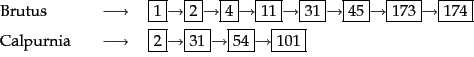
\includegraphics[scale=0.6]{pics/invFile.png}
	\caption{Inverted Index}
\end{figure}



}
\end{frame}



\begin{frame}\frametitle{Web Search Engines [1]}


{\footnotesize
  A search engine is an information retrieval system designed for searching information on the Web (solving information needs) \cite{manning2008}. Its basic components are:  

\begin{block}


\begin{itemize}
\item Crawler: a robot that navigates the Web according to a defined strategy. It usually starts by browsing a set of seed websites and continues to browse their hyperlinks.
\item Indexer: in charge of maintaining an inverted index with the content of the pages traversed by the Crawler.
\item Query processor: in charge of processing user queries and searching the index for the documents most relevant to a query.
\item Ranking function: the function used by the query processor to rank documents indexed in the collection by relevance according to a query.
\item User interface: receives the query as input and returns the documents ranked by relevancy.
\end{itemize}

\end{block}
}

\end{frame}


\begin{frame}\frametitle{Web Search Engines [2]}

\begin{figure}[h!]
	\centering
	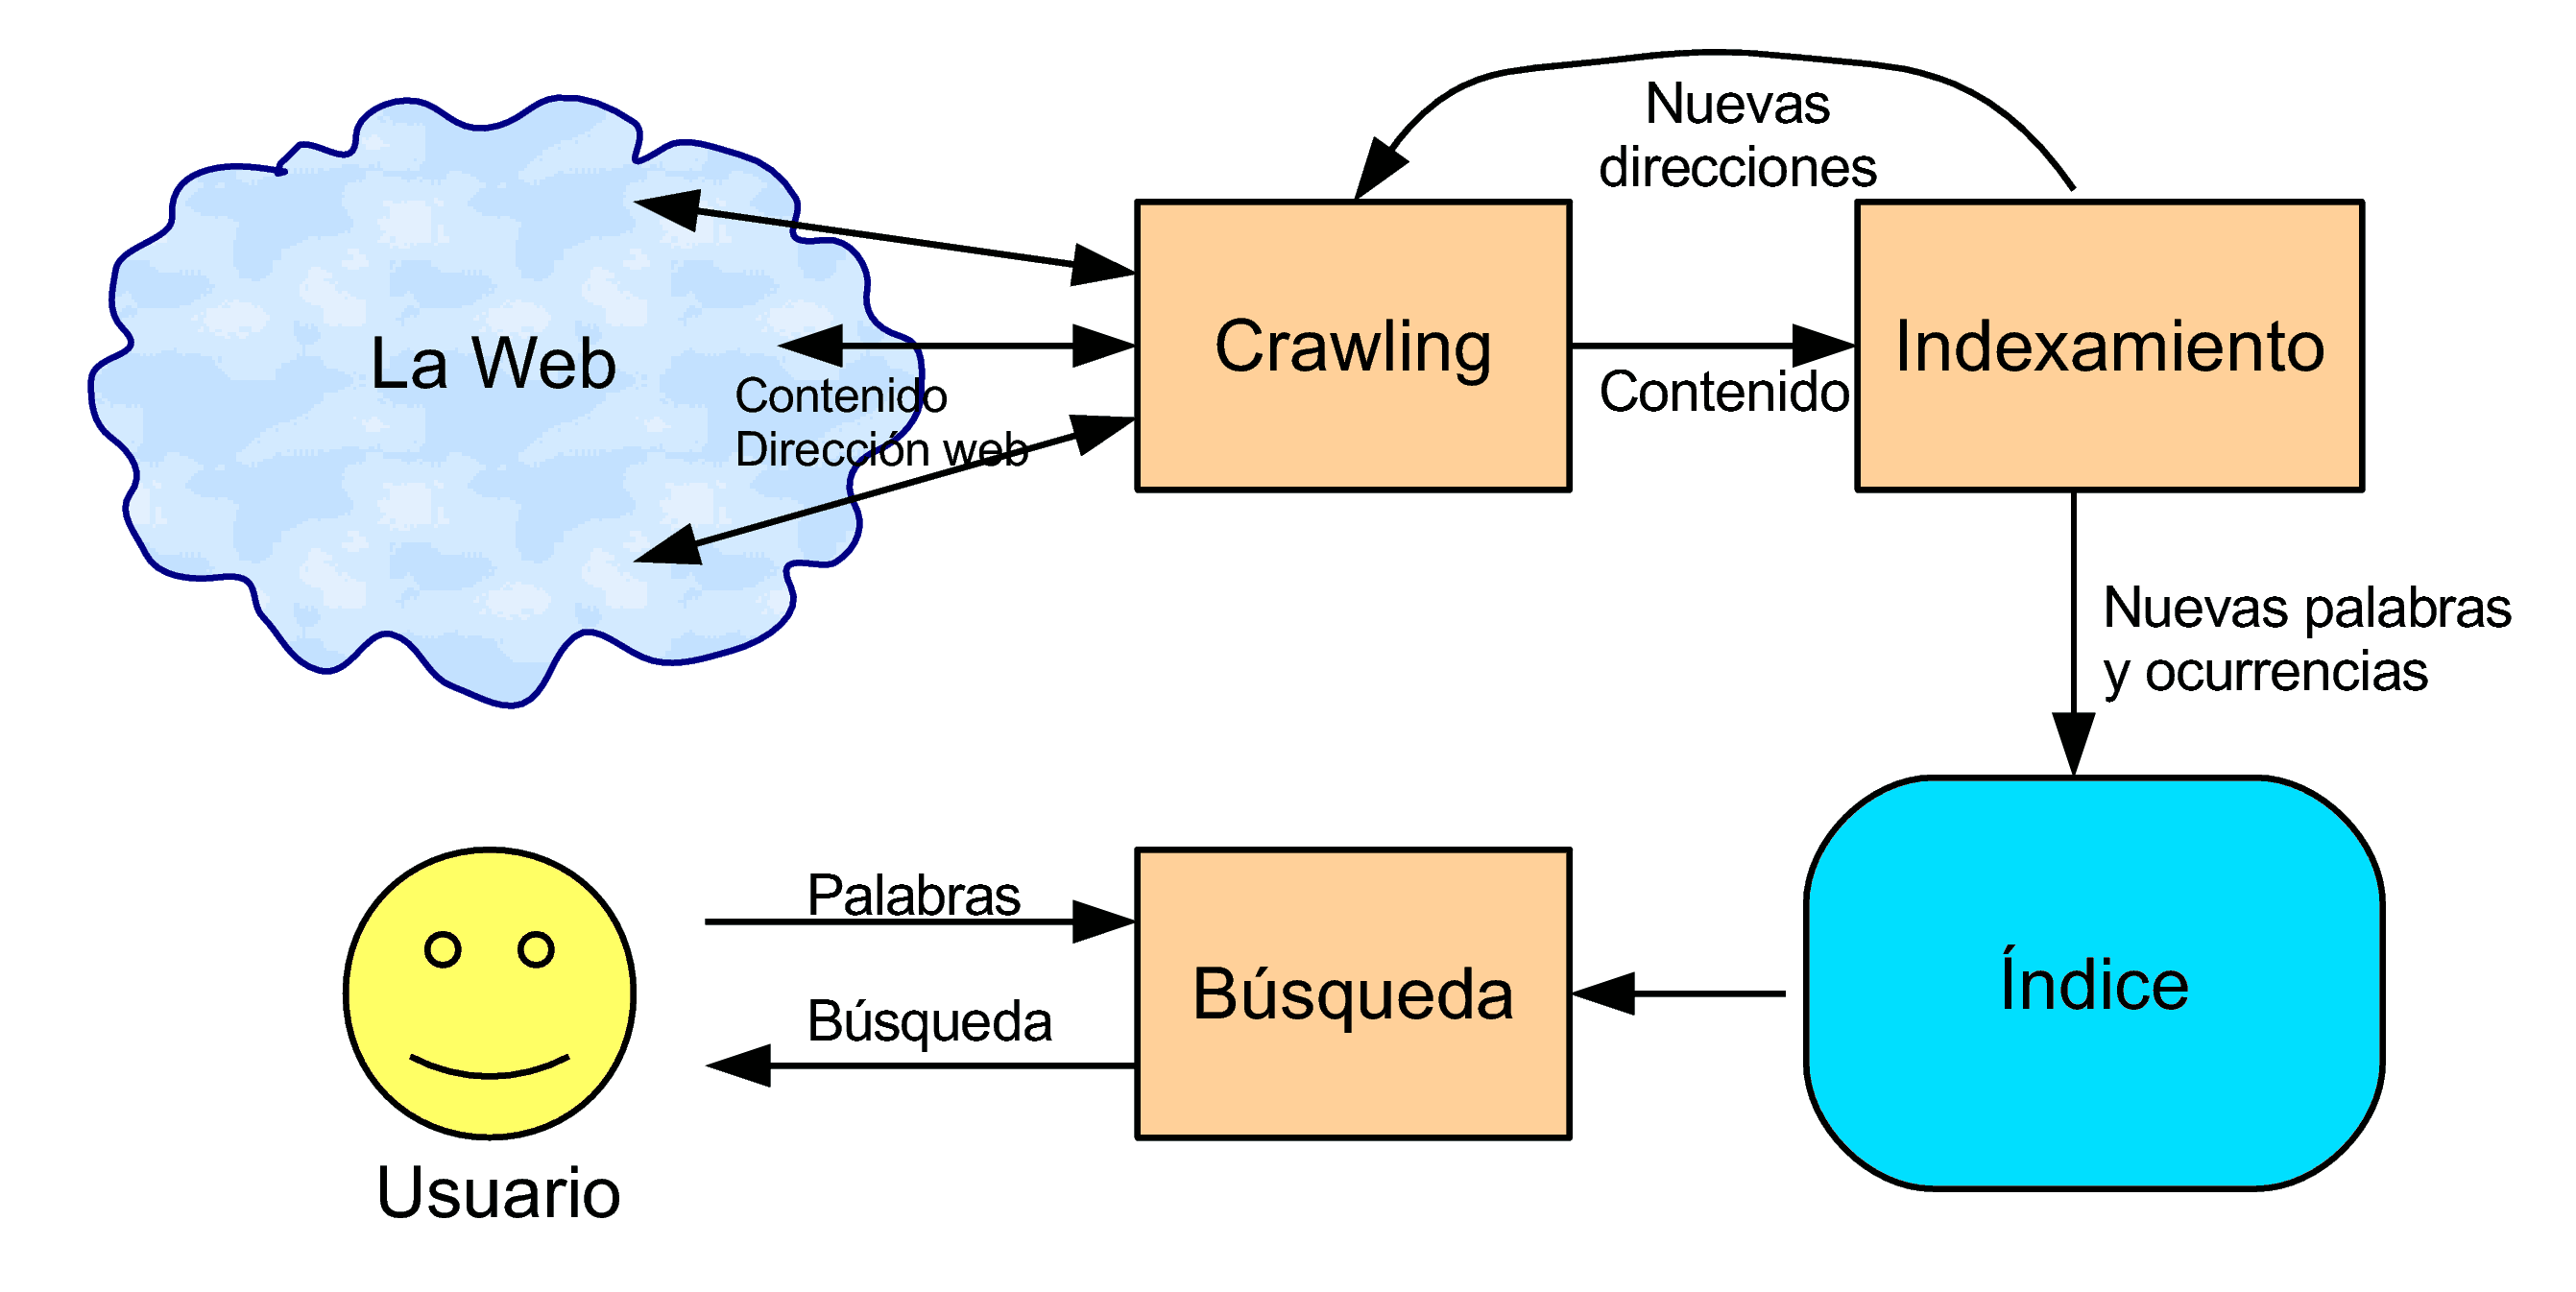
\includegraphics[scale=0.25]{pics/searchengine.png}
	\caption{ The various components of a web search engine~\cite{manning2008}.}
\end{figure}

\end{frame}

\begin{frame}\frametitle{The Vector Space Model}
\footnotesize{
\begin{itemize}
 \item In order to rank queries, or measure the similarity between two documents we need a similarity metric.
 \item Documents can be \textit{represented} as vectors of terms, where each term is a vector dimension \cite{salton1975vector}. 
 \item Documents with different words and lengths will reside in the same vector space.
 \item These types of representations are called \emph{Bag of Words}.
 \item In bag-of-words-representations the order of words and the linguistic structure of a sentence is loss. 
 \item The value of each dimension is a weight that represents the relevance of the term $t_{i}$ in the document $d$.

\begin{equation}
 d_{j} \rightarrow \overrightarrow{d_{j}}=(w(t_{1},d_{j}),...,w(t_{|V|},d_{j}))
\end{equation}

\item How can we model how informative is a term to a document?
 
\end{itemize}

}
 
\end{frame}

\begin{frame}\frametitle{Term Frequency - Inverted Document Frequency [1]}
\footnotesize{
\begin{itemize}
 \item Let $tf_{i,j}$ be the frequency of term $t_{i}$ in document $d_{j}$.
 \item A term that occurs $10$ times should provide more information than one that occurs once.
 \item  What happens when we have documents that are much longer than the others?
 \item We can normalize by the maximum term frequency in the document. 
\begin{displaymath}
 ntf_{i,j}=\frac{tf_{i,j}}{\max_i (tf_{i,j})}
\end{displaymath}
\item  Does a term that occurs in very few documents provide more or less information than one that occurs several times?
\item For example, the document \emph{The respected major of Pelotillehue}. The term \emph{Pelotillehue} occurs in fewer documents than the term \emph{major}, so it should be more descriptive. 
\end{itemize}


} 
\end{frame}

\begin{frame}\frametitle{Term Frequency - Inverted Document Frequency [2]}
\footnotesize{ 
\begin{itemize}
 \item Let $N$ be the number of documents in the collection and $n_{i}$ the number of documents containing term $t_{i}$, we define $idf$ of $t_{i}$ as follows: 
 \begin{displaymath}
  idf_{t_{i}}= log_{10}(\frac{N}{n_{i}})
 \end{displaymath}
\item A term that appears in all documents would have $idf=0$ and one that appears in $10\%$ of the documents would have $idf=1$.

\item The $tf$-$idf$ scoring model combines $tf$ and $idf$ scores, resulting in the following weights $w$ for a term in a document:
\begin{displaymath}
w(t_{i},d_{j})=tf_{i}\times log_{10}(\frac{N}{n_{i}}) 
\end{displaymath}

\item Search engine queries can also be modeled as vectors. However, queries have  between $2$ and $3$ terms in average. To avoid having too many null dimensions, query vectors can be smoothed as follows:
\begin{displaymath}
 w(t_{i},d_{j})=(0.5+0.5\times tf_{i,j})log_{10}(\frac{N}{n_{i}}) 
\end{displaymath}



\end{itemize}



}

\end{frame}

\begin{frame}\frametitle{Similarity between Vectors}
\footnotesize{
\begin{itemize}
 \item Representing queries and documents as vectors allows calculating their similarity.
 \item One approach would be using the euclidean distance.
 
 \item The common approach is to calculate the cosine of the angle between the two vectors.
 \item If both documents are the same, the angle would be $0$ and its cosine would be $1$. On the other hand, if they are orthogonal  the cosine is $0$.
 \item The cosine similarity is calculated as follows:
 \begin{displaymath}
 cos(\vec{d}_{1},\vec{d}_{2})= \frac{\vec{d}_{1}\cdot \vec{d}_{2}}{|\vec{d}_{1}|\times|\vec{d}_{2}|} = \frac{\sum_{i=1}^{|V|}(w(t_{i},d_{1})\times w(t_{i},d_{2}))}{\sqrt{\sum_{i=1}^{|V|} w(t_{i},d_{1})^2}\times \sqrt{\sum_{i=1}^{|V|} w(t_{i},d_{2})^2}}
\end{displaymath}
\item This is wrongly called \emph{cosine distance}. It is actually a similarity metric.
\item Notice that cosine similarity normalizes the vectors by its euclidean norm $||\vec{d}||_{2}$.

\end{itemize}


}
\end{frame}

\begin{frame}{Cosine Similarity}

\begin{figure}[h!]
	\centering
	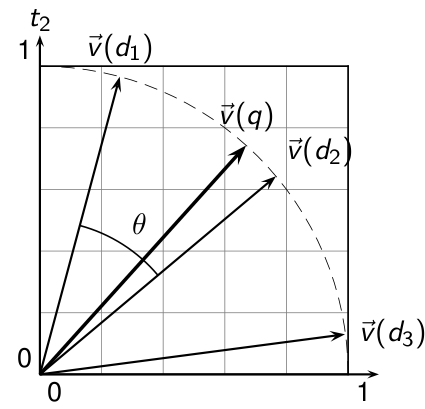
\includegraphics[scale=0.5]{pics/cos.png}
	\caption{ Cosine Similarity.}
\end{figure}

\end{frame}

\begin{frame}{Exercise}
\begin{itemize}
 \item Suppose we have $3$ documents formed from the following sequences of terms: \\
 $d_{1}\rightarrow t_{4}t_{3}t_{1}t_{4}$ \\
 $d_{2}\rightarrow t_{5}t_{4}t_{2}t_{3}t_{5}$ \\
 $d_{3}\rightarrow t_{2}t_{1}t_{4}t_{4}$ \\

\item Build a term-document matrix of $5\times3$ dimensions using simple $tf$-$idf$ weights (without normalization).
\item  We recommend you first build a list with the number of documents in which each term appears (useful for calculating $idf$ scores) 
\item Then calculate the $idf$ scores of each term.
\item Fill up the cells of the matrix the $tf$-$idf$ values.
\item Which is the closest document to $d_{1}$?
\end{itemize}


\end{frame}

\begin{frame}{Result}
 \begin{table}[htbp]
\caption{tf-idf Matrix}
\begin{tabular}{|l|r|r|r|}
\hline
 & \multicolumn{1}{l|}{d1} & \multicolumn{1}{l|}{d2} & \multicolumn{1}{l|}{d3} \\ \hline
t1 & 0.176 & 0.000 & 0.176 \\ \hline
t2 & 0.000 & 0.176 & 0.176 \\ \hline
t3 & 0.176 & 0.176 & 0.000 \\ \hline
t4 & 0.000 & 0.000 & 0.000 \\ \hline
t5 & 0.000 & 0.954 & 0.000 \\ \hline
\end{tabular}
\end{table}

\end{frame}

\begin{frame}{Document Clustering [1]}
\footnotesize{
\begin{itemize}
 \item How can we group documents that are similar with each other?
 \item Clustering is the process of grouping documents that are similar with each other.
 \item Each group of documents is called a \emph{cluster}. 
 \item In clustering we try to identify groups of documents in which the similarity between documents in the same cluster is maximized and the similarity of documents in different clusters is minimized.
\begin{figure}[h!]
	\centering
	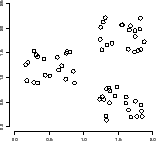
\includegraphics[scale=0.6]{pics/cluster.png}
	\caption{ Set of documents where the clusters can be clearly identified.}
\end{figure}
 
\end{itemize}


}
 
\end{frame}

\begin{frame}{Document Clustering [2]}
\footnotesize{
\begin{itemize}
 \item Document clustering allows identifying topics in a corpus and reducing the search space in a search engine i.e., the inverted index is organized according to the clusters. 
 \item K-means is a simple clustering algorithm that receives the number of clusters $k$ as a parameter.
 \item The algorithm relies on the idea of \emph{centroid}, which is the average vector of documents belonging to the same cluster.
 \item Let $S$ be a set of $2$-dimensional vectors $\{3,6\}, \{1,2\}, \{5,1\}$, the centroid of $S$ is $\{(3+1+5)/3,(6+2+1)/3\} = \{3,3\}$.

\end{itemize}
}
\end{frame}


\begin{frame}{K-Means}
\footnotesize{
    \begin{enumerate}
    \footnotesize{
    \item We start with $k$ random centroids.
    \item We calculate the similarity between each document and each centroid.
    \item We assign each document to its closest centroid forming a cluster.
    \item The centroids are recalculated according to the documents assigned to them.
    \item This process is repeated until convergence.}
    \end{enumerate}

}
\end{frame}


\begin{frame}{K-means}
\begin{figure}[h!]
	\centering
	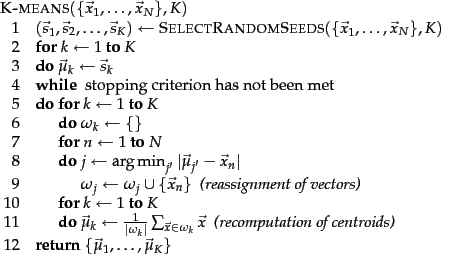
\includegraphics[scale=0.6]{pics/kmeans.png}
	\caption{ K-means algorithm}
\end{figure}

 
\end{frame}

\begin{frame}\frametitle{Conclusions and Additional Concepts}
\footnotesize{
\begin{itemize}
 \item Representing documents as vectors is essential for calculating similarities between document pairs.
 \item Bag of words vectors lack linguistic structure.
 \item Bag of words vectors are high-dimensional and sparse. 
 \item Word n-grams can help capturing multi word-expressions (e.g., New York $=>$ new\_york)
 \item Modern information retrieval systems go beyond vector similarity (PageRank, Relevance Feedback, Query log mining, Google Knowledge Graph, Machine Learning).
 \item Information retrieval and text mining are less concerned with linguistic structure, and more interested in producing fast and scalable algorithms \cite{jacobbook}. 
\end{itemize}


}
\end{frame}



\begin{frame}[allowframebreaks]\scriptsize
\frametitle{References}
\bibliography{bio}
\bibliographystyle{apalike}
%\bibliographystyle{flexbib}
\end{frame}



%%%%%%%%%%%%%%%%%%%%%%%%%%%

\end{document}
